\section{Tuning the hyperparameters}
Note that the default value of \textit{num\_trees} is 300, and \textit{max\_depth} is 16.
\subsection{Random Forests Tuning}
\subsubsection{Number of Trees}
We experimented with the number of trees in the Random Forest, keeping max-depth as the default value, i.e. 16\\
\begin{figure}[htbp]
    \centering
    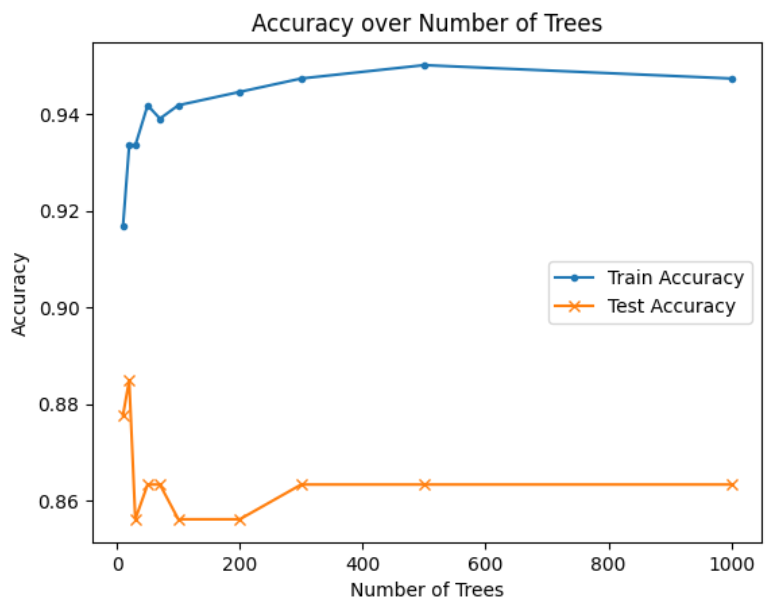
\includegraphics[width=0.8\linewidth]{images/rf_acc_num_trees.png}
    \caption*{Train and test accuracy against varying number of trees}
    \label{fig:your_label}
\end{figure}\\
Here, we observe that after a point, both training and testing accuracy stop increasing.
\newpage
\subsubsection{Max-depth}

We experimented with the  max-depth in the Random Forest, keeping nunber of trees as 500, fixed. This is obtained by observing the previous graph. Here are the results of the experiment.\\
\begin{figure}[htbp]
    \centering
    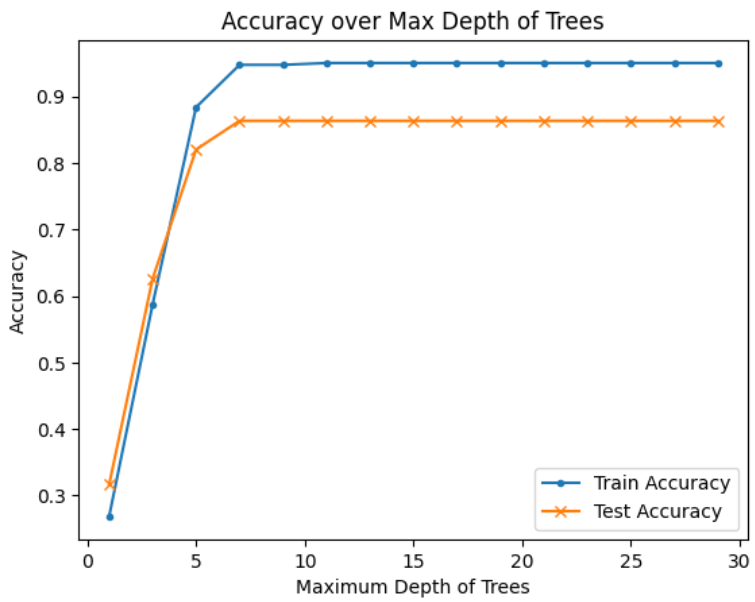
\includegraphics[width=0.8\linewidth]{images/rf_acc_max_depth.png}
    \caption*{Train and test accuracy against varying max-depth}
    \label{fig:your_label}
\end{figure}
\newline
We can see that when the number of trees reach 7, the accuracy values settle. Keeping a smaller number also helps in avoiding overfitting. Also, initially due to extremely small depth, the model is underfitted and the train accuracy is even lower than the test accuracy.

\newpage
\subsection{Gradient Boosted Decision Tree Tuning}
\subsubsection{Number of Trees}
We experimented with the number of trees, keeping max-depth as 15\\
\begin{figure}[htbp]
    \centering
    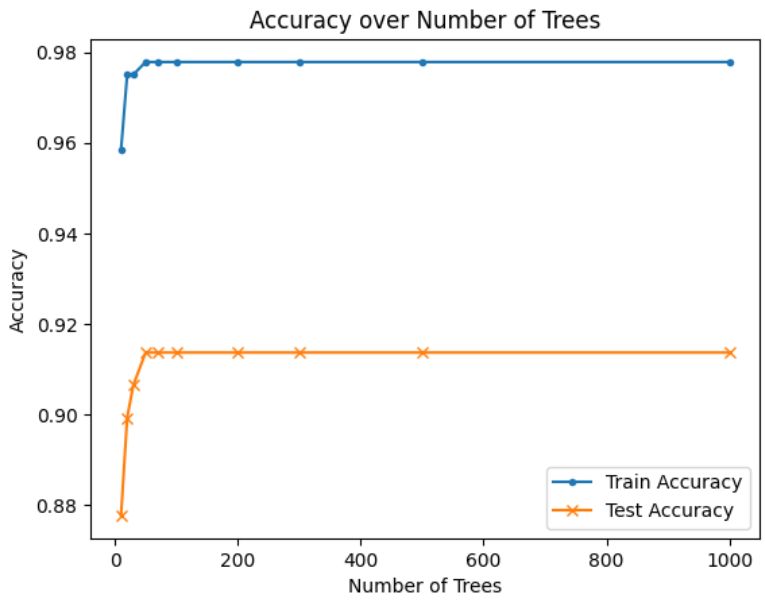
\includegraphics[width=0.58\linewidth]{images/gbdt_acc_num_trees1.png}
    \caption*{Train and test accuracy against varying number of trees}
    \label{fig:your_label}
\end{figure}
\newline
We observe that in case of GBDT, the accuracies plateau faster as compared to RF. So, we test again, but on more \textt{num\_trees} values between 0 and 100. Here are the results:

\begin{figure}[htbp]
    \centering
    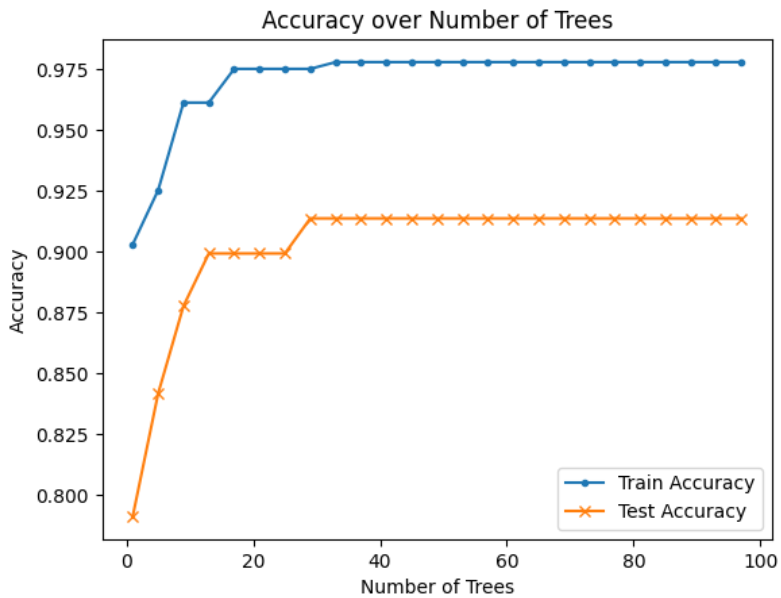
\includegraphics[width=0.6\linewidth]{images/gbdt_acc_num_trees2.png}
    \caption*{Train and test accuracy against varying number of trees}
    \label{fig:your_label}
\end{figure}

Note that for \texttt{num\_trees} till 30, the accuracy increases, and thereafter, it becomes mostly constant

\subsubsection{Max-depth}
We experimented with the  max-depth in the Random Forest, keeping number of trees as 30, fixed. This is obtained from previous graph.\\
\begin{figure}[htbp]
    \centering
    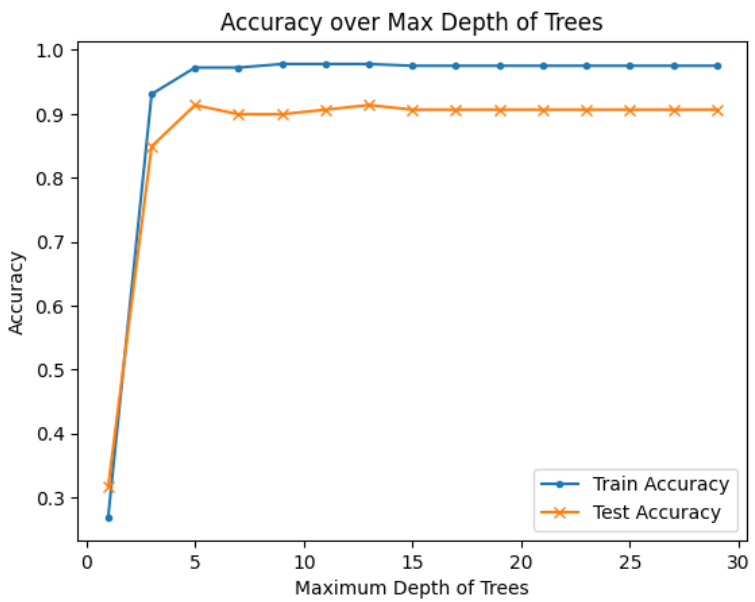
\includegraphics[width=0.8\linewidth]{images/gbdt_acc_max_depth.png}
    \caption*{Train and test accuracy against varying max-depth}
    \label{fig:your_label}
\end{figure}
\newline
The accuracy increases with increasing max-depth till 5, then a slight stagnation.
It becomes maximum at around 14, and then decreases due to overfitting. Here too, initially the model is underfitted due to extremely small depth.\\


\newpage
\subsection{Final Models with Reasonable Accuracy}

This section presents the final hyperparameters which achieve a reasonable accuracy over the given dataset.

\subsubsection{{Random Forest (RF)} model}

Hyperparameters:
\begin{itemize}
    \item \texttt{num\_trees}: 500
    \item \texttt{max\_depth}: 9
\end{itemize}}  

\textbf{RF Accuracy}: 
\begin{itemize}
    \item Train = 94.73\%, 
    \item Test = 86.33\%
\end{itemize}

\bigskip

\subsubsection{Gradient Boosted Decision Tree (GBDT) model}

Hyperparameters:
\begin{itemize}
    \item \texttt{num\_trees}: 30
    \item \texttt{max\_depth}: 5
\end{itemize}}  

\textbf{GBDT Accuracy}: 
\begin{itemize}
    \item Train = 97.72\%, 
    \item Test = 91.36\%
\end{itemize}


Hence, it can be seen that Gradient Boosted Random Trees achieve a better accuracy than Random Forests at much smaller costs, i.e. it requires much less number of trees and less maximum-depth to achieve it.